%!TEX root = thesis.tex

\chapter{Introduction}
\label{chap:intro}

The success of the technological advances often can be associated with an unprecedented convenience that they bring in. At the heart of 
this convenience lies the ability to relax the limitations of the human body to a certain extent. From this point of view, it is not a 
surprise that the three most prominent technological wonders of the last century, namely the \emph{Television}, the \emph{Telephone} and 
the \emph{Radio} (which was originally called \enquote{radiotelegraphy}), bears the same Greek prefix \emph{tele-} which corresponds to 
\enquote{\emph{at a distance}} in our context. This shows that there is something of extreme importance about our drive to extend our 
capabilities beyond the constraints that our bodies impose.


It is quite remarkable, in retrospect, that these \enquote{gadgets} did not perish but rather kept on evolving since, initially, they were 
far from perfect. Quite to the contrary, they were hardly operational. Even the commercialized version of the early TVs had a narrow 
bandwidth and minimum image quality. Similarly radio and telephone was barely transmitting sensible information as far as the 
signal-to-noise ratio is concerned. Nevertheless, they have provided the ways of communication which were unimaginable before their time. Therefore 
the added value dominated the shortcomings and even though they were quite imperfect, we kept using them. The important lesson to be 
learned is that a technology should not be judged by its imperfections, but rather should be weighed by its contribution in this context 
and the convenience that is either immediately brought in by using it, or its foreseen potential by the \enquote{early adopters}. 
%In fact
%the following quote is attributed to Herbert E. Ives\footnote{Best known for the famous \enquote{Ives-Stillman experiment} for showing the 
%relativistic time-dilation effect .}
%\begin{displayquote}
%Many technical problems have yet to be solved before television can claim to be more than an interesting novelty and 
%it remains for the future to disclose what its field of utility will be.
%\end{displayquote}
\begin{figure}
\begin{subfigure}[b]{.3\linewidth}
\centering%
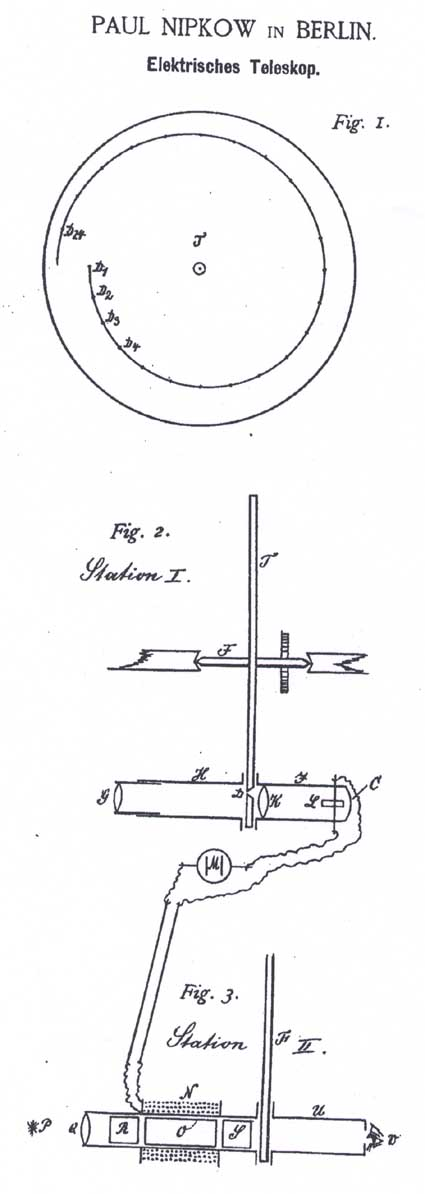
\includegraphics[height=5cm]{\impath/intro/nipkowdisc}%
\caption{}
\label{fig:intro:nipkow}
\end{subfigure}%
\begin{subfigure}[b]{.65\linewidth}
\centering%
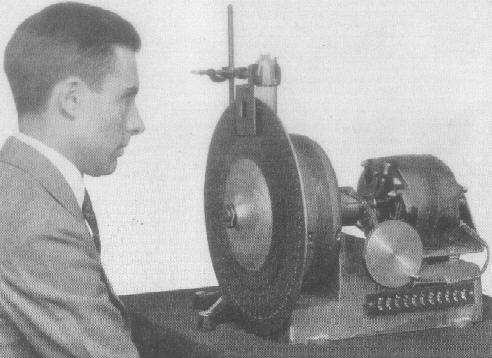
\includegraphics[height=5cm]{\impath/intro/watchtv}%
\caption{}
\label{fig:intro:watchtv}
\end{subfigure}
\caption[Some historical details from the early mechanical television era]%
{Some historical details from the early mechanical television era: (a) Nipkow disc from Paul Gottlieb Nipkow's patent application, 
(b) Watching Television in 1928; the rotating perforated disc has 50 holes spirally placed, and rotates 18 times a second. Images are 
from \cite{nipkow,watchtv} respectively.%
}
\label{fig:intro:mechtv}
\end{figure}


The success is also related to the fact that these technologies mainly relied on the human brain itself at their early stages. For 
example, the human brain did most of the noise filtering and data recovery by just guessing the missing pieces and identifying patterns 
from the signal brought by the respective medium. Today, with our smart mobile phones and 3D LED TVs, we can assume that the 
computational load, or whatever its equivalent in terms of attention span capacity, on the human brain is drastically reduced. In other 
words, it is true that we are still identifying patterns and utilizing the relevant parts of our brain to make sense of a TV broadcast\footnote{Pun 
intended.}. However, we do not need to use a higher level of concentration to reconstruct the words that we hear or to identify the image 
on the display thanks to the high quality output. We cannot exaggerate the importance of the human brain and its immersion power. 

We are on the same track and leaving essentially the same footprints with the technological developments involving our touch sense. 
Though various science fiction items already used such ideas extensively, the real technology tends to follow from quite a distance.  
Considering the importance of our sense of touch in any given situation, the added value of extending our perception in this modality 
needs no motivation. Take the most familiar, the vibrating mobile phone in the silent mode in our pocket. This is a very important 
example since every individual learns what that vibration might mean, either an SMS or a call, depending on the vibrational pattern. This 
means that the sense of touch can be used to convey messages that are not immediately related to physical act of touching. More 
importantly we can process those messages for inference which forms the basis of the so-called \enquote{haptics} and haptic technology.


The type of information from the cell-phone example is said to be received via the haptic channel (or the collaborative use of tactile 
and proprioceptive modalities). At this point we have to emphasize that, we use the term \enquote{sense of touch} rather vaguely as a 
shortcut and we leave it to the experts of the field to define the sophisticated mechanisms (pertaining to the somatosensory system) that 
we utilize when we manipulate objects, say with our bare hands. 


Since our skin and muscles form one of most sophisticated and complex sensory systems, the somatosensory system, the brain can easily 
interpret the slightest changes and this extra signal processing power gives us a chance to hack into this system by providing artificial 
inputs via haptic displays. Still, it is rather conspicuous that it is impossible to achieve a total immersion with today's technology. 
The essential complication is twofold: the high sensitivity of the very same sensory system makes it difficult to fake or mimic a natural 
phenomenon by artificial means and on the other hand we do not have a well-defined mapping from the to-be-created sensation to the 
required excitation signals. Moreover, even if we have such mappings available, the related hardware must execute the computed haptic 
signal profiles perfectly which is generally not the case and a trade-off strategy should be constructed. In other words, we need a clear 
approximation metric to be able to compare two different touch technologies to judge whether one is better than the other. Unfortunately, 
this metric and thus the strategy is also absent. 
 
Then, we could simply ask \emph{Why bother?} 


\section{The Objectives}
\label{sec:intro:obj}

We first give a summary about the current concepts of the involved technology (as we foresee from a narrow \enquote{today's} perspective). 
Later on, we define our microscopic focus of this thesis within this vast generality. This would provide additional insights to what follows 
in the later sections.  


Touch related applications are diverse. The diversity is not only in terms of the sensation they are related to (texture, shape etc.) but 
also how they encode the information and transmit via various modalities (e.g. vibrational patterns in mobile electronics, variable 
resistance to motion in game consoles and steering wheels etc.). There is no particular reason to limit ourselves with the daily needs or 
even luxurious demands regarding our touch sense as mobile phones taught us that a vibration in our pocket means a contact request from 
someone which is hardly ever related to the touch sense. It should be pretty awkward to experience if someone actually would come and 
shake our pockets to draw our attention (unless it is socially accepted). Therefore, we have devised a way to translate one particular 
message into another by simply teaching ourselves and getting used to it. Thus, it does not seem improbable that other types of physical 
measurements in terms temperature, light intensity etc., converted into pressure or tactile patterns in time domain.

Hence, it is our belief that the crux of this technology is establishing a interpretable protocol between our brain and the machine but 
not exactly reflecting the particular state of some distant or virtual physical medium. 
This would be the main argument of this thesis when we distinguish our approach with its comparable counterparts. For this reason, we 
have identified the nuances in \Cref{chap:apdxphysio} to narrow down our focus further by defining different types of touch related 
concepts.



\subsubsection{Bilateral Teleoperation}

Bilateral teleoperation, simply, is teleoperation equipped with force feedback to the human operator with the hope to increase the realism 
by recreating the force vectors of the distant medium at the local environment. The majority of the bilateral teleoperation research is 
devoted to kinesthetic feedback. In particular, the human interacts with the local device by moving a constrained handle to explore the 
environment or using a stylus-like stick. Hence, the experience is mostly based on the success of imitating a physical tool. Therefore, 
the tactile cues are of secondary nature. The challenge, of course, is to increase the performance level to a tactile display level while 
still maintaining the tool usage capability. The particular MIS tasks that are performed with a scalpel are one of the hot topics of 
research effort. It requires not only kinesthetic feedback, though a major accomplishment by itself, but tactile feedback too, for 
understanding the nature of the texture or the stiffness of the tissue. Similarly, teleoperated peg-in-hole type of tasks are also a major 
area of investigation; e.g., ground-satellite robotic mission directives or underwater construction tasks would benefit much from such 
possibilities to reduce the operational cost, duration, and success rate. 



There are many interesting challenges when it comes to this recreation process. For example, in a microassembly task, the experienced 
forces are substantially different from what we feel during daily tasks. Gravity is our main source of reference when interpreting a 
distant location. However, gravity becomes almost negligible in the micro domain, as adhesive forces such as Van der Waals, electrostatic 
and surface tension forces dominate --- the most common example is that the the parts that are picked up in microdomain 
tend to stick to the tweezers. Similarly in a space- or underwater- operation, there might be different forces that are not directly 
visible/interpretable by vision alone, say underwater currents or relative forcing between free bodies in space etc.

If we manage to create a believable level of force feedback sensation in these otherwise inaccessible domains, there are a few very 
important quasi-philosophical and also task-dependent questions that need to be answered. A few of these questions are:

\begin{itemize}
	\item Should the device reflect the unfamiliar forces to the human operator for the sake of realism which are utterly counter-%
intuitive and even worse appear to be happening at random? 
    \item Is there any correlation between increased realism and increased comfort? In case of a difficult task, what good does the 
    realism bring in by replicating the difficult task at a distant location in the local environment?
    \item Do we need to reflect the human motion to the remote location perfectly since this can be considered as a waste of resources? 
    In other words, we neglect the fact that a robot can perform certain tasks much more precisely than a human operator. Is there any 
    downsampling/upsampling protocol to vary the motion precision depending on the receiver?
    \item If we decide to filter the irrelevant force information (e.g., mental/muscular fatigue, tremor on the operator side and 
    measurement noise, nonlinear effects  on the remote device side), how should we know what to transmit and what to filter out? 
    \item Do we use the full capacity of our \emph{internal data bus} to transfer touch information, or put differently, is there any 
space left to encode other quantities on top of the touch sense?
    \item Can we assume that all users more or less reach to the same understanding given a kinesthetic cue sequence?
\end{itemize}

These are interesting questions and answering them in a rigorous fashion is very challenging. The reason for enumerating a few of 
them here is that the problem is much more involved than what we can achieve within the scope of this thesis. In other words, we 
cannot, despite the recurring claims found in the literature, answer these questions within the scope of control theory/robotics alone. 
Instead we will focus on a framework that would help to set up such teleoperation devices such that experts in the involved fields 
can use these devices to answer those items above. 



\subsection{Structure and Objectives of this Thesis}
To restrict the scope of this thesis further, we exclusively stay in bilateral teleoperation concept as we have defined it previously (via 
the classification given in \Cref{chap:apdxphysio}) and focus on the control theoretical aspects of the teleoperation for a stable 
interaction with sufficient performance levels. The reason of such a terminological classification is to precisely draw the boundaries of 
what will follow in the later chapters. Such a restriction is necessary to keep the discussion of the involved approaches/methodologies 
mutually exclusive which are often presented in a rather intertwined fashion in the literature.

In \Cref{chap:litsurvey}, we first give an opinionated version of the literature to point out to the underlying connections between 
seemingly different methodologies and also provide an arguably simpler explanation of the well-known \emph{wave variables} formalism. By 
doing so, we classify such methods in the corresponding mainstream control theory methods and demonstrate that they are indeed outdated in 
the light of the recent advances. Moreover, we argue that the by-now-standard assumption of \emph{passivity} property on the human and 
environment is not experimentally validated. We also claim that the success of passivity-based methods are due to the conservatism 
of these tests and not due to the validity of the assumption.

In a similar fashion, in \Cref{chap:perf}, we enumerate the available performance objectives by which we should design bilateral 
teleoperation systems proposed in the literature. Then we argue why these objectives might not be valid candidates for the problem at hand.

In \Cref{chap:analysis}, we also show both theoretically and numerically that the frequency domain methods (and a limited number of 
nonlinear methods) found in the literature can be combined under one framework via \emph{Integral Quadratic Constraints} (IQCs). With these 
results, we demonstrate that the proposed approach of this thesis does not bring in additional complications or conservatism. In fact, 
via numerical case studies, we show that the results are precisely the same with those of the techniques available in the literature.
Therefore, there is no fundamental reason to use a specialized terminology of the networks and microwave systems which in turn alienates 
mainstream control theory experts. We also remark that uncertainty modeling is a key aspect in obtaining better controllers for bilateral 
teleoperation. To highlight the reasons why we promote this framework, we also give examples of different combinations of uncertainties 
for which classical tools that are employed in the teleoperation literature are not suitable but already available in the robust control 
literature for almost two decades. 


After establishing this link with the methods in the literature, we turn to the controller synthesis problem in \Cref{chap:synth}. We 
formulate the problem as a generalized plant and work out the scarce details that are found in the literature to obtain a better model-
based control synthesis algorithm using static and dynamic IQCs. For the interested reader, we also explicitly identify what the 
implementation-related bottlenecks are. Then, in \Cref{chap:application}, we utilize this framework to design controllers for an experimental 
setup.

In \Cref{chap:conc}, we provide some concluding remarks and for the reader's convenience, in \Cref{chap:apdxnetwork}, we recap the basics 
of the network theory.
\newpage
Let us turn to our initial question \enquote{\emph{Why Bother?}}. We do because there is no need to obtain the ultimate, perfect touch sensation for 
the human in order to interpret the signals correctly. It is the same principle with LED TVs. Nowhere on the screen, a color different 
than red, green, or blue is emitted. However, we tend to approximate the combined output of the closely positioned RGB LED triplets to 
the closest color since the distance between the emitters are negligible for the viewer and we achieve the color perception. Therefore, 
realism is not our primary objective. However, before we can even enter the discussion of what leads to a satisfactory sense of touch, 
we need to make sure that the teleoperation devices, i.e., our tools that we actually try to understand the sense of touch with, are 
stable and exhibit consistent performance such that experts from neuroscience, psychophysiology, and other related scientific fields can 
join and assess different ways of protocolling with the human brain in this modality. Otherwise their conclusions would be contaminated 
by the device properties. We can even speculate that this is often the case, though no proof will be presented here.  


Thus the precise goal of this thesis is first to show the state-of-art control problems in the literature regarding the bilateral 
teleoperation with a critical evaluation of the claims often found in various studies. Then, we consider the stability properties and 
control problem of bilateral teleoperation without fully understanding the underlying problem. Unlike many sources in the literature, we 
openly discuss the reasons behind the lack of understanding and clearly point out the vague performance objectives reported in the 
literature. The method adopted here and the application to an experimental setup constitute yet another stab at problem from a pure 
engineering/applied mathematics point-of-view. To the best of our knowledge, it is a superior methodology if compared to the existing 
literature in the sense that the uncertainties and perturbations can be handled more systematically while defining performance objectives. 
Moreover, the resulting performance verifies the methodology and theoretical claims. However, this is not enough to argue that we have 
actually set up a beneficial and widely applicable framework that leads to a stable and high-performance bilateral teleoperation systems. 

In other words, it should be obvious that the methodology given here does not contribute to infer far-reaching conclusions about the 
human-perception or the nature of the bilateral teleoperation problem. Instead it only solves the problem of setting up a system that 
achieves robust operation specifications under the apparent and strictly limited understanding of what bilateral teleoperation might require. 
